\section{Pianificazione del lavoro}
La prima riunione del gruppo � avvenuta il giorno 13 luglio presso la facolt� d'ingegneria di Brescia. Calendario alla mano abbiamo iniziato a pianificare l'attivit� di valutazione del sito web scelto; valutando l'ampia disponibilit� di tempo libero nella pausa estiva e considerando i vari impegni sia personali che universitari, abbiamo ritenuto plausibile di completare il lavoro per la sessione d'esame di dicembre/gennaio. Non era stata stabilit� una data precisa in quanto non era ancora stata fissata alcuna data d'esame per tale periodo.\\
Una volta definita una simbolica data di terminazione, stabilita per l'8 dicembre abbiamo iniziato il lavoro di pianificazione dell'attivit�, avvalendoci come strumento di aiuto, del diagramma di Grantt abbiamo cercato di pianificare tutte le fasi del progetto.\\
\newline
\begin{figure}[!h]
\centering
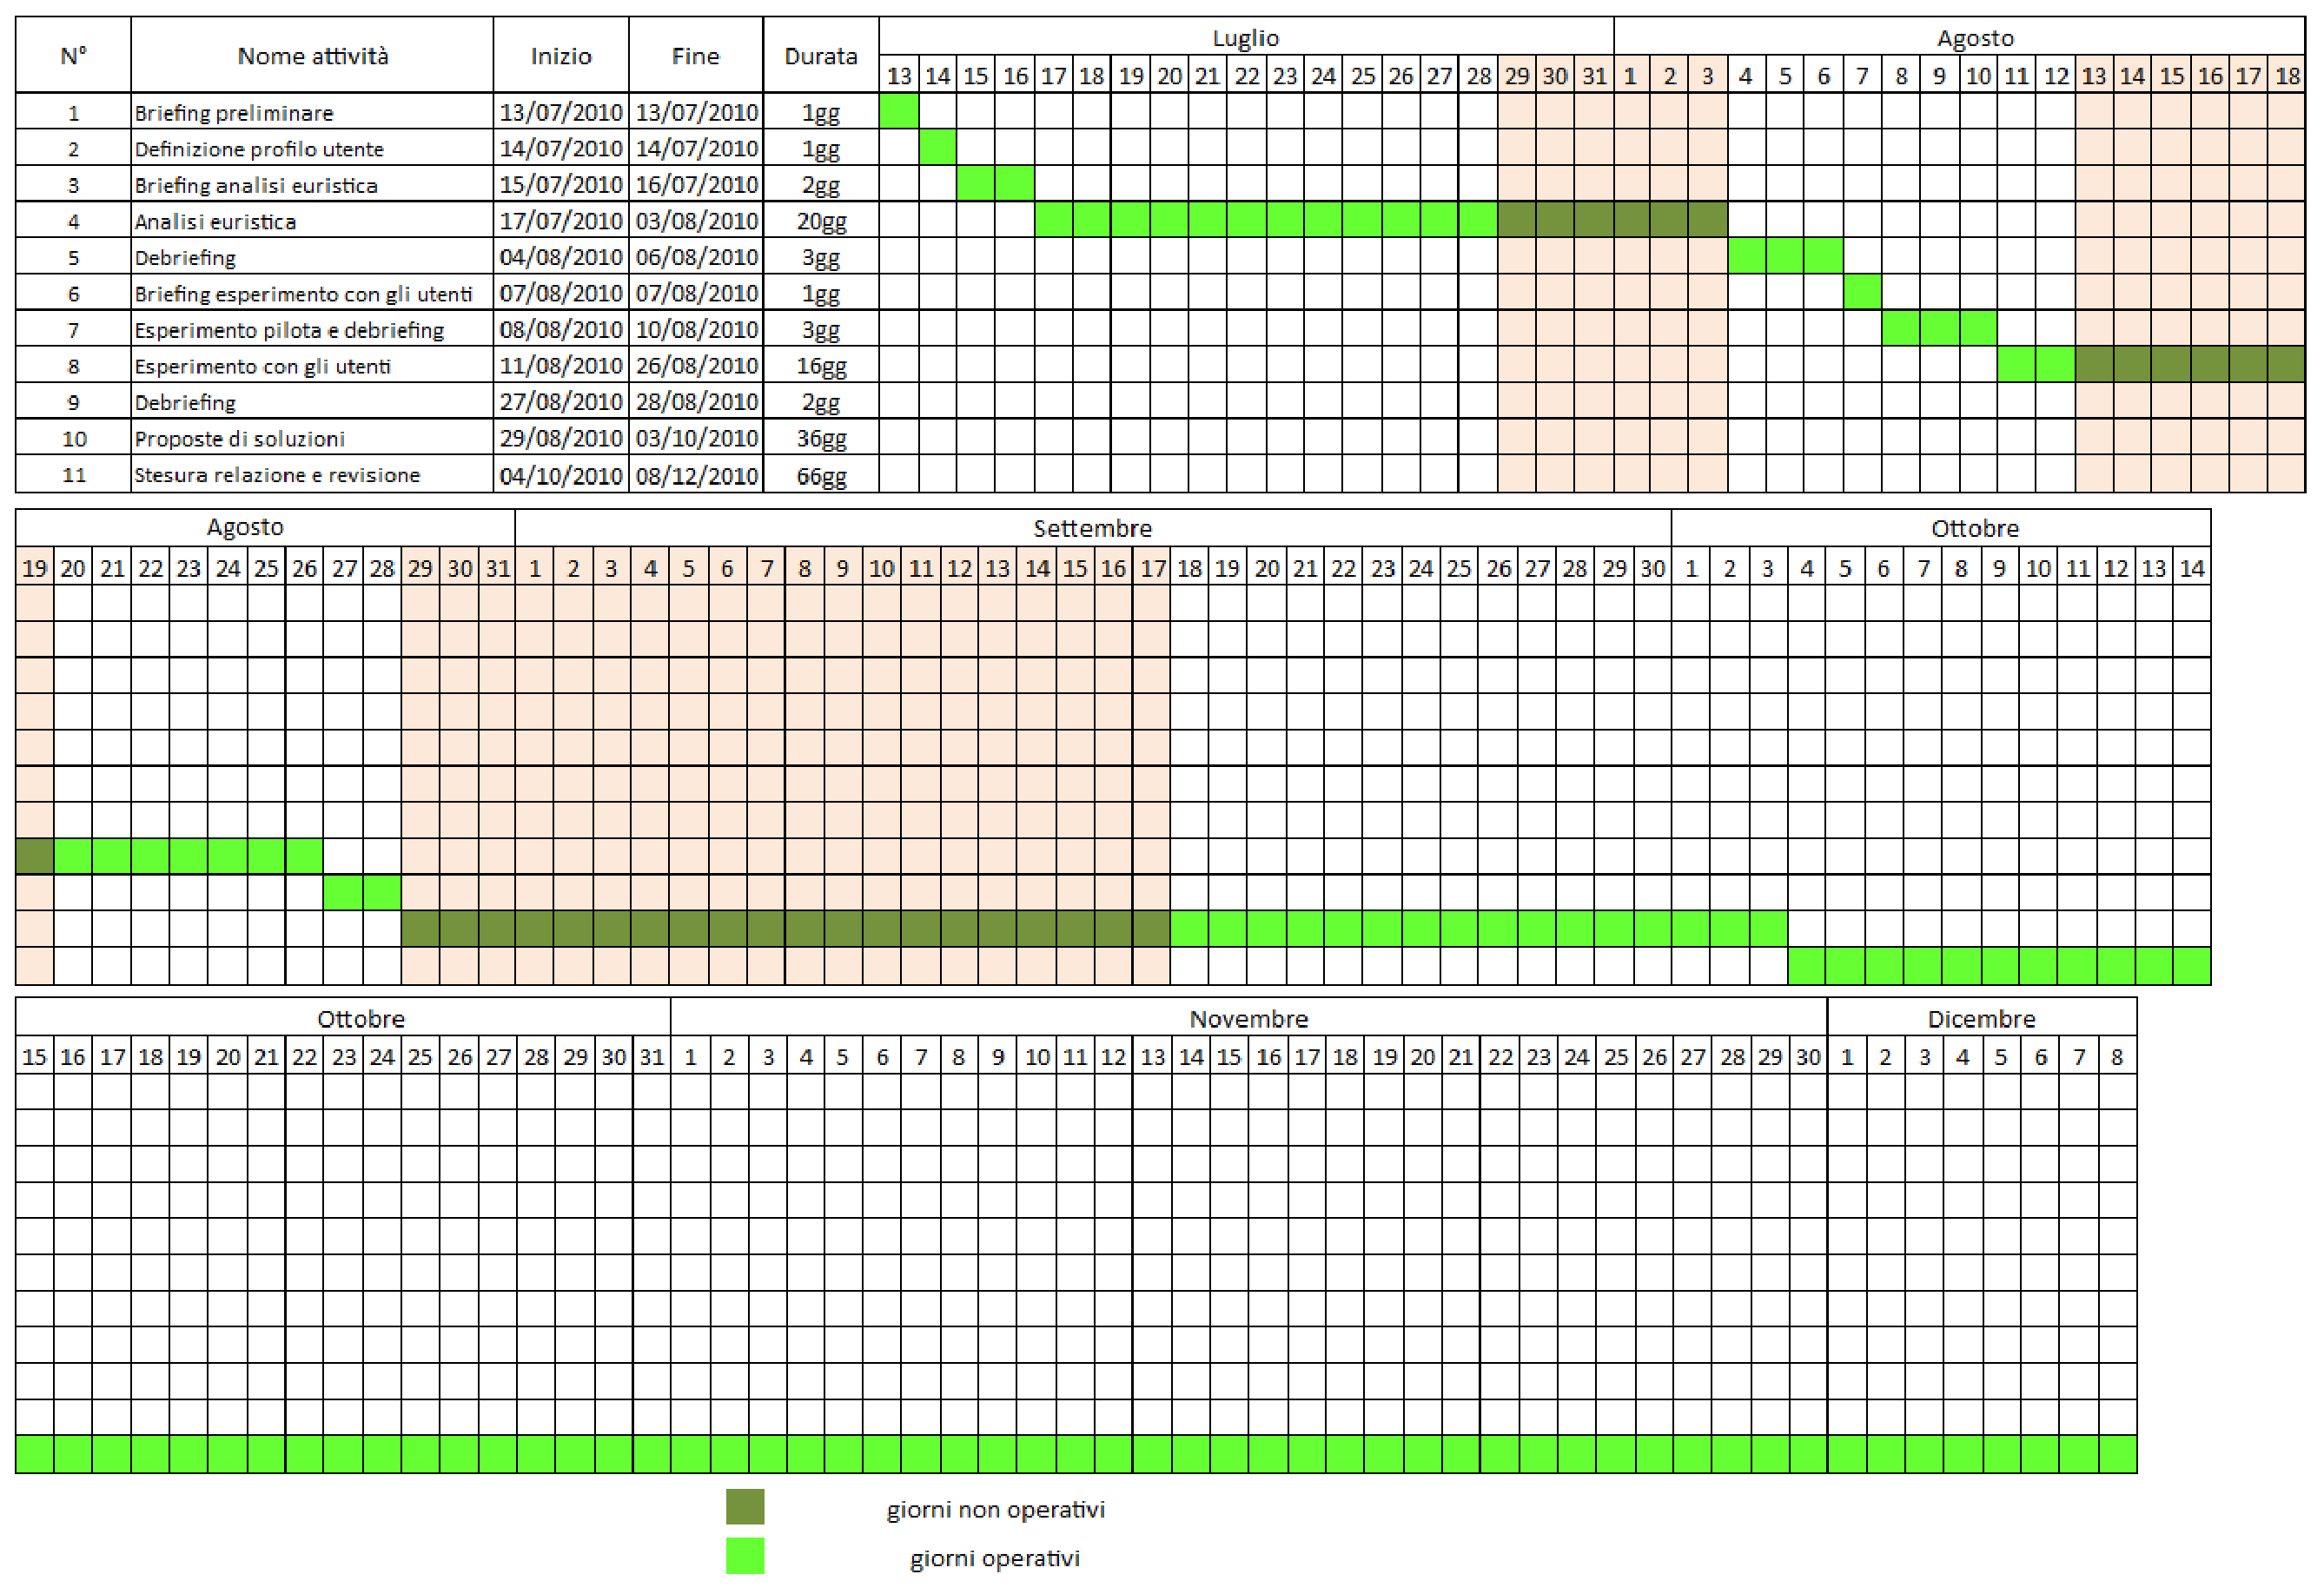
\includegraphics[angle=90,scale=0.52]{figure/grantt.eps}
\caption{Grafico di Grantt per la pianificazione del lavoro}
\label{fig:grantt}
\end{figure}
A causa d'impegni imprevisti sia di carettere universitario che lavorativo, il diagramma di Grantt mostrato in figura \ref{fig:grantt} � rimasto una mera idea, e tutte le tempistiche hanno subito grossi ritardi e slittamenti, anche di parecchie settimane; tali ritardi sono da imputare a guasti imprevisti, esami e impegni di lavoro. In particolare le fasi ``Debriefing'' dopo l'esperimento con gli utenti e le ``Proposte di soluzioni'' hanno subito i maggiori ritardi. La stesura della relazione ha richiesto pi� tempo di quanto preventivato, in quanto gli impegni dei membri del gruppo non consentivano di avere dei summit regolari, per verificare l'effettivo stato di avanzamento del progetto. 
